\section{Physics goals}
We will measure the differential cross section for the charged-current (CC) interaction on $\mathrm{H_2O}$ and Hydrocarbon(CH)).
The water-scintillator mass ratio of the WAGASCI module is as high as 4:1 and the high purity measurement
of the cross section on $\mathrm{H_2O}$ is possible.
One experimental option is to remove water from one of the two WAGASCI modules. 
The water-out WAGASCI module will allow to measure pure-CH target interactions with very low momentum-threshold for protons.
It will also benefit to subtract the background from interaction with scintillator in the water target measurement.
Another option is to add the T2K proton module which is fully made of plastic scintillators.
It will allow the high statistics comparison of cross section between $\mathrm{H_2O}$ and CH and also comparison
with the ND280 measurement. The actual configuration will be optimized with detailed MC simulation by 2018 Summer.

Our setup allows the measurements of inclusive and also exclusive channels such as
$1\mu$, $1\mu 1p$, 1$\mu 1\pi^\pm \mathrm{n}p$ samples, former two of which are mainly caused by the quasi-elastic and
2p2h interaction and the latter is mainly caused by resonant or coherent pion production and deep elastic scattering.
In general, an accelerator produced neutrino beam spectrum is wide and the energy reconstruction
somehow rely on the neutrino interaction model.
Therefore, recent neutrino cross section measurement results including those from T2K are given
as a flux-integrated cross section rather than cross sections as a function of the neutrino energy to avoid bias from the model.
We can provide the flux-integrated cross section.
In addition, by combining our measurements with those at ND280, model-independent extraction of the cross section
for narrow neutrino energy spread becomes possible.
This method was demonstrated in \cite{Abe:2015biq} and also proposed by the E61 (NUPRISM) experiment.

\subsection{Expected number of events}
Expected number of CC neutrino events remaining after the event selections was evaluated with simulation.
Detailes are described in Sec.~\ref{sec:mc_study}.
In neutrino-mode, 5,400, 1,100 and 3,800 events are expected for the water-in WAGASCI module, the water-out WAGASCI module and the INGRID proton module with $5\times 10^{20}$ POT.  Among 5,400 events for the water-in WAGASCI module,78~\%  are interactions on $\mathrm{H_2O}$.
In the antineutrino-mode, 2,240, 400 and 1,500 CC antineutrino events are expected for the water-in WAGASCI module, the water-out WAGASCI module and the INGRID proton module with $5\times 10^{20}$ POT. Amongh 2,240, 74~\% are interactions on $\mathrm{H_2O}$.
The wrong-sign interactions in antineutrino-mode is 561 events, but will be removed with 90~\% or higher efficiency by Baby MIND.

%Statical errors of flux integrated CC-inclusive neutrino cross section measurements on H$_{2}$O (full acceptance) and CH targets (forward acceptance)
%will be 1.5 \% and 1.6 \% with $5\times 10^{20}$ POT in the neutrino-mode.
%Statical errors of flux integrated CC-inclusive antineutrino cross section measurements on H$_{2}$O (full acceptance) and CH targets (forward acceptance)
%will be 2.4 \% and 2.5 \% with $5\times 10^{20}$ POT in the antineutrino-mode.


%Statical errors of flux integrated H$_{2}$O to CH CC-inclusive neutrino cross section ratio measurement 
%will be 3.1 \% (full acceptance) and 2.3 \% (forward acceptance) with $5\times 10^{20}$ POT in the neutrino-mode.
%Statical errors of flux integrated H$_{2}$O to CH CC-inclusive antineutrino cross section ratio measurement will be 5 \% (full acceptance) and 3.7 \% (forward acceptance) with $5\times 10^{20}$ POT in the antineutrino-mode.

\subsection{Pseudo-monochromatic beam by using different off-axis fluxes}
The off-axis method gives narrower neutrino spectrum, and the peak energy is lower for larger off-axis angle.
There still remains a high energy tail mainly due to neutrinos from Kaon decay.
The off-axis angle of the WAGASCI location is 1.5 degree and different from the ND280 2.5 degree.
Top two plots of Fig.~\ref{fig:fluxsubtfhc} show the energy spectra of fluxes and neutrino interaction events
at these two different locations.
By using the WAGASCI measurement results, the high energy tail of ND280 flux can be somehow subtracted.
The low energy part of the WAGASCI flux can be also subtracted by using the ND280 measurement.
Bottom two plots of Fig.~\ref{fig:fluxsubtfhc} demonstrate this method.
We can effectively get two fluxes, from 0.2 GeV to 0.9 GeV and 0.6 GeV and 2 GeV
and measure flux-integrated cross section for these two fluxes.
It should be noted that even though the statistical errors are drawn for each energy bin for the bottom right plot of Fig.~\ref{fig:fluxsubtfhc},
measurement results will be given as an integration across energies.

\begin{figure}[tbhp]
\begin{center}
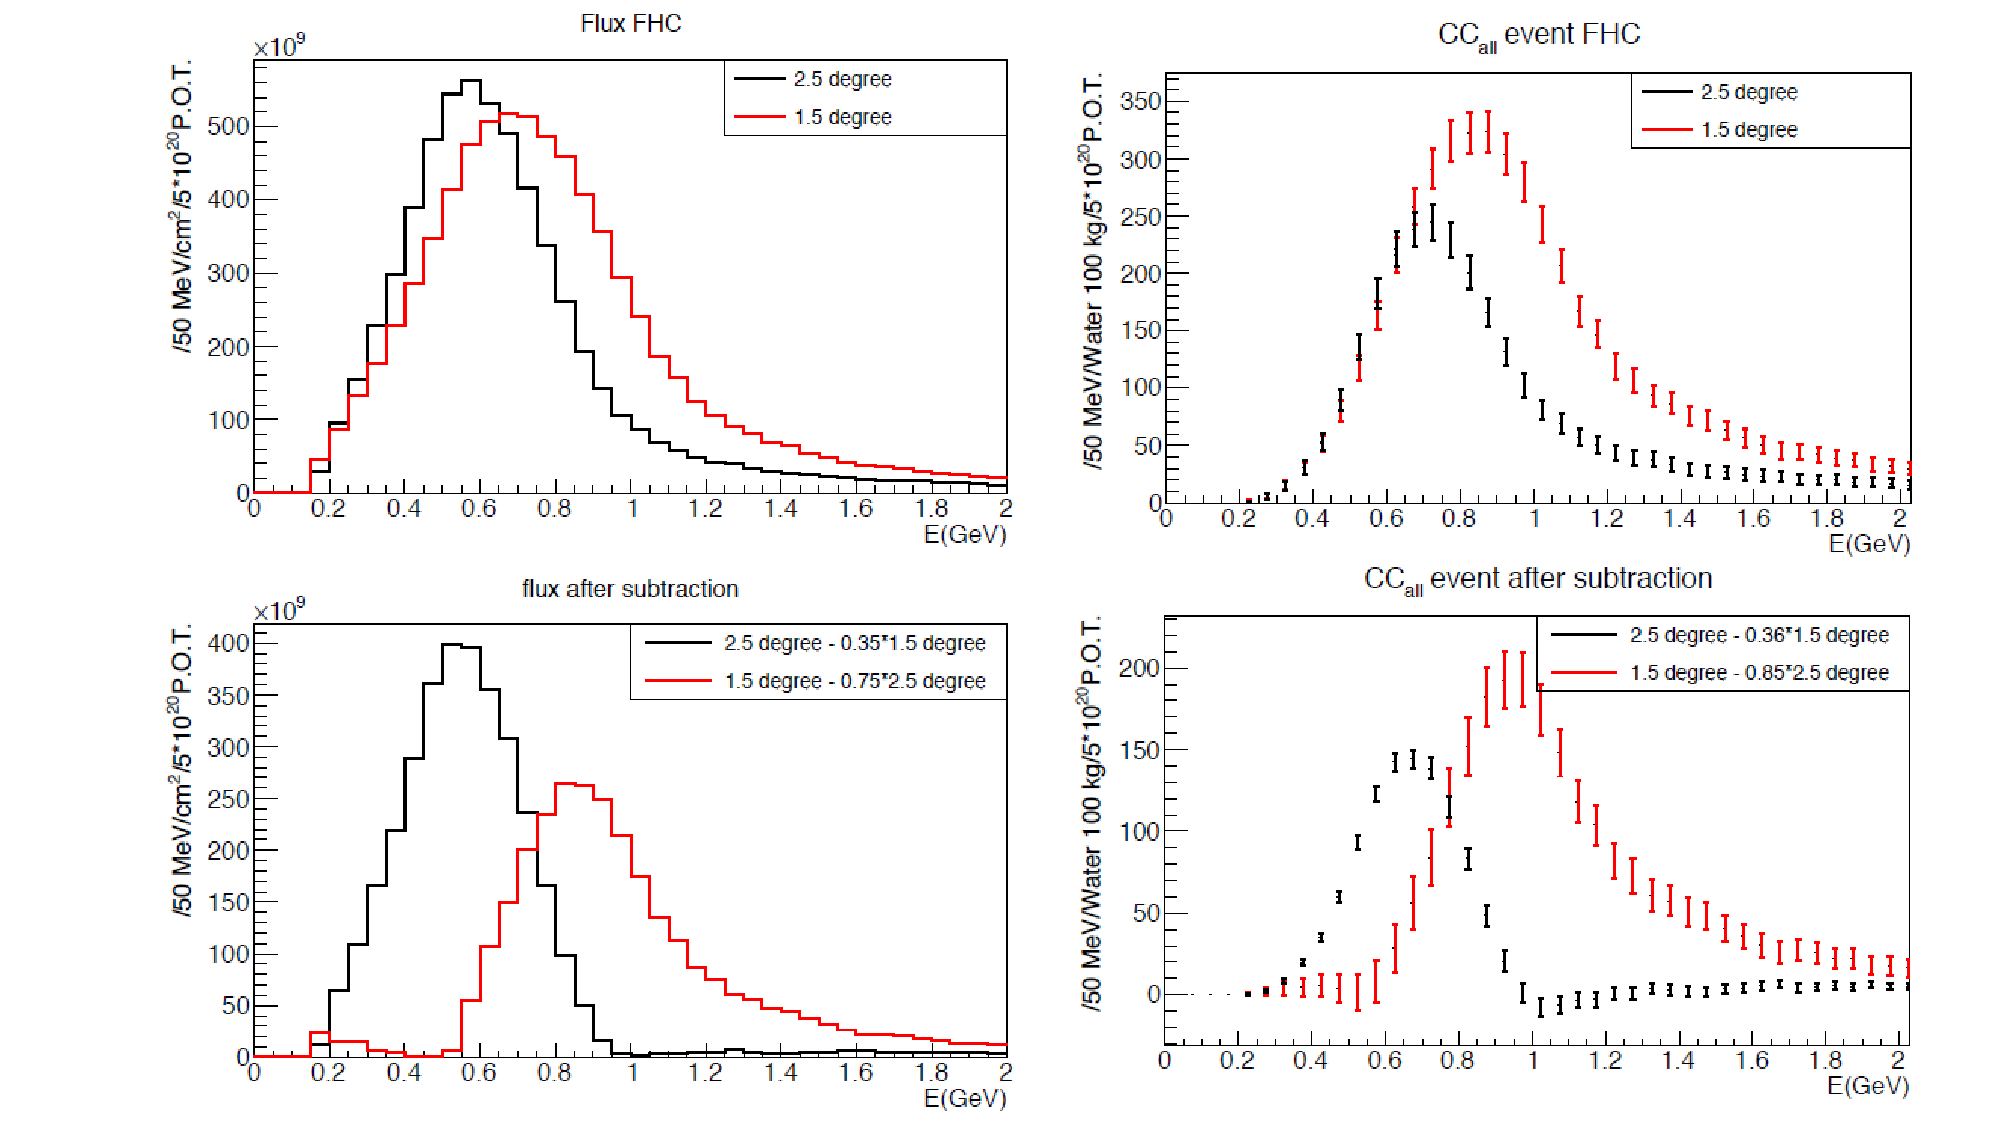
\includegraphics[width=\textwidth]{fig/fluxsubtractFHC.pdf}
\end{center}
\caption{Energy spectra obtained by using different off-axis angle fluxes.
  Top two plots show the fluxes(left) and spectra of interaction events (right) for ND280 (off-axis 2.5 degree) and WAGASCI (off-axis 1.5 degree). Bottom two plots show the fluxes (left) and spectra of interaction events (right) obtained by
  subtraction of fluxes at ND280 and WAGASCI.
  The error bar is for the statistical error and those in the bottom right plot is obtained assuming the statistical error
  for the ND280 measurement is much smaller than that of the WAGASCI experiment.
}
\label{fig:fluxsubtfhc}
\end{figure}


%Statical errors of flux integrated CC-inclusive neutrino cross section measurements on H$_{2}$O (forward acceptance) and CH targets (forward acceptance) with the pseudo-monochromatic beam
%will be 2 \% and 1.9 \% with $5\times 10^{20}$ POT in the neutrino-mode.
%Statical errors of flux integrated CC-inclusive antineutrino cross section measurements on H$_{2}$O (forward acceptance) and CH targets (forward acceptance) with the pseudo-monochromatic beam
%will be 3 \% and 2.8 \% with $5\times 10^{20}$ POT in the neutrino-mode.

\subsection{Extraction of Cross sections}
The flux-integrated CC inclusive cross sections on $\mathrm{H_2O}$ and CH are calculated from the number of selected events
with background subtraction and efficiency correction
\begin{equation*}
\sigma_{CC} = \frac{N_{sel}-N_{BG}}{\phi T \epsilon},
\end{equation*}
where $N_{sel}$ is the number of selected events from the real data,
$N_{BG}$ is the number of contaminated background events,
$\phi$ is the integrated $\nu_{\mu}$ flux, $T$ is the number of target nucleons,
and $\epsilon$ is the detection efficiency for signal estimated by MC simulation.
The number of main background events is effectively estimated from side-band samples.
The CH interaction background for the $\mathrm{H_2O}$ measurement is estimated from the measurement of the Water-out WAGASCI module and/or
the proton module.
The neutrino interaction background for the antineutrino measurement is estimated from the opposite-sign interactions selected by Baby MIND.
% The $\nu_{\mu}$ CC inclusive cross sections on water and hydrocarbon are measured from the number of selected events
%in the water and hydrocarbon regions in the central detector.
% The $\nu_{\mu}$ CC inclusive cross section ration on water to hydrocarbon is measured 
% using the two results.
The dominant error for the inclusive total cross section measurement is the uncertainty of the neutrino flux, which is $\sim$9\% now and is expected to be reduced to $\sim$6\%.
Since the flux error is dominated by the normalization type error,
the flux error can be significantly reduced for the relative comparison of the $\mathrm{H_2O}$ and CH cross sections
and the relative comparison of the ND280 and WAGASCI measurements.
For example, T2K INGRID succeeded to determine the cross section ratio for CH and Fe with 3\% precision\cite{ingrid_ccinclusive}.
For the exclusive and/or differential corss section measurements, statistical error would be dominant, size of which depending on the binning.

\subsection{Subjects WAGASCI can contribute}
Recent accelerator neutrino experiments use nuclear target e.g. organic scintillator, water and iron.
So the interaction is largely affected by nuclear effects such as Fermi motion, correlated pairs of nucleons in nucleus (two particles-two holes, 2p2h), collective nuclear effects 
%calculated with Random Phase Approximation (RPA) 
and final state interactions (FSI) of secondary particles in the nuclei after the initial neutrino interactions.

The main interaction type at the T2K energy (sub GeV) is the CC quasi-elastic (CCQE) interaction with nucleons inside nucleus.
The energy is reconstructed from the lepton momentum assuming CCQE kinematics in T2K and other interactions would bias the reconstructed energy.
Figure~\ref{fig:ene_rec_bias} shows how the reconstructed energy is affected.
The 2p2h interactions mainly happen through the interaction with a correlated nucleons pair and also through the $\Delta$ resonance interaction
followed by pion-less decay.
The 2p2h interactions are observed in electron scattering experiments \cite{escattering} where the 2p2h events were observed in the gap between quasi-elastic region and pion-production region.% as shown in Fig. \ref{fig:electrono_scattering_data}.
Neutrino experiments have attempted to measure the 2p2h interactions, but so far there are only indicative results because the energy spectrum of the neutrino beam is wide and the precision of the event-by-event determination of the neutrino energy is not good nor suffered from bias.
%separation of the QE peak and the 2p2h peak is more difficult because transferred momentum (p) and energy (w) are largely affected by  neutrino energies which cannot be determined event-by-event in the wide energy spectrum of the accelerator neutrino beam.
Our measurements, when combined with ND280 measurement, will give the cross section values for narrow energy-spread fluxes
and give insight for such interactions. 
%Our model-independent narrow neutrino spectra extracted from combined analyses of our data and ND280 data are ideal for searching the 2p2h interaction because clearer separation of the QE peak and the 2p2h peak is expected.
Another efficient way to investigate the 2p2h interaction is direct measurement of proton tracks with low momentum threshold and wide acceptance.
Figure~\ref{fig:2p2h_proton_multiplicity_angle} left plot shows proton multiplicities for the CCQE events and 2p2h events.
Figure~\ref{fig:2p2h_proton_multiplicity_angle} right plot shows opening angles of two proton-tracks for the events having two protons.
The water-out WAGASCI can provide good sample for the 2p2h interaction search because its low density medium enables the detection of low momentum protons in side acceptance.
%
%\begin{figure}[tbh]
%\begin{center}
%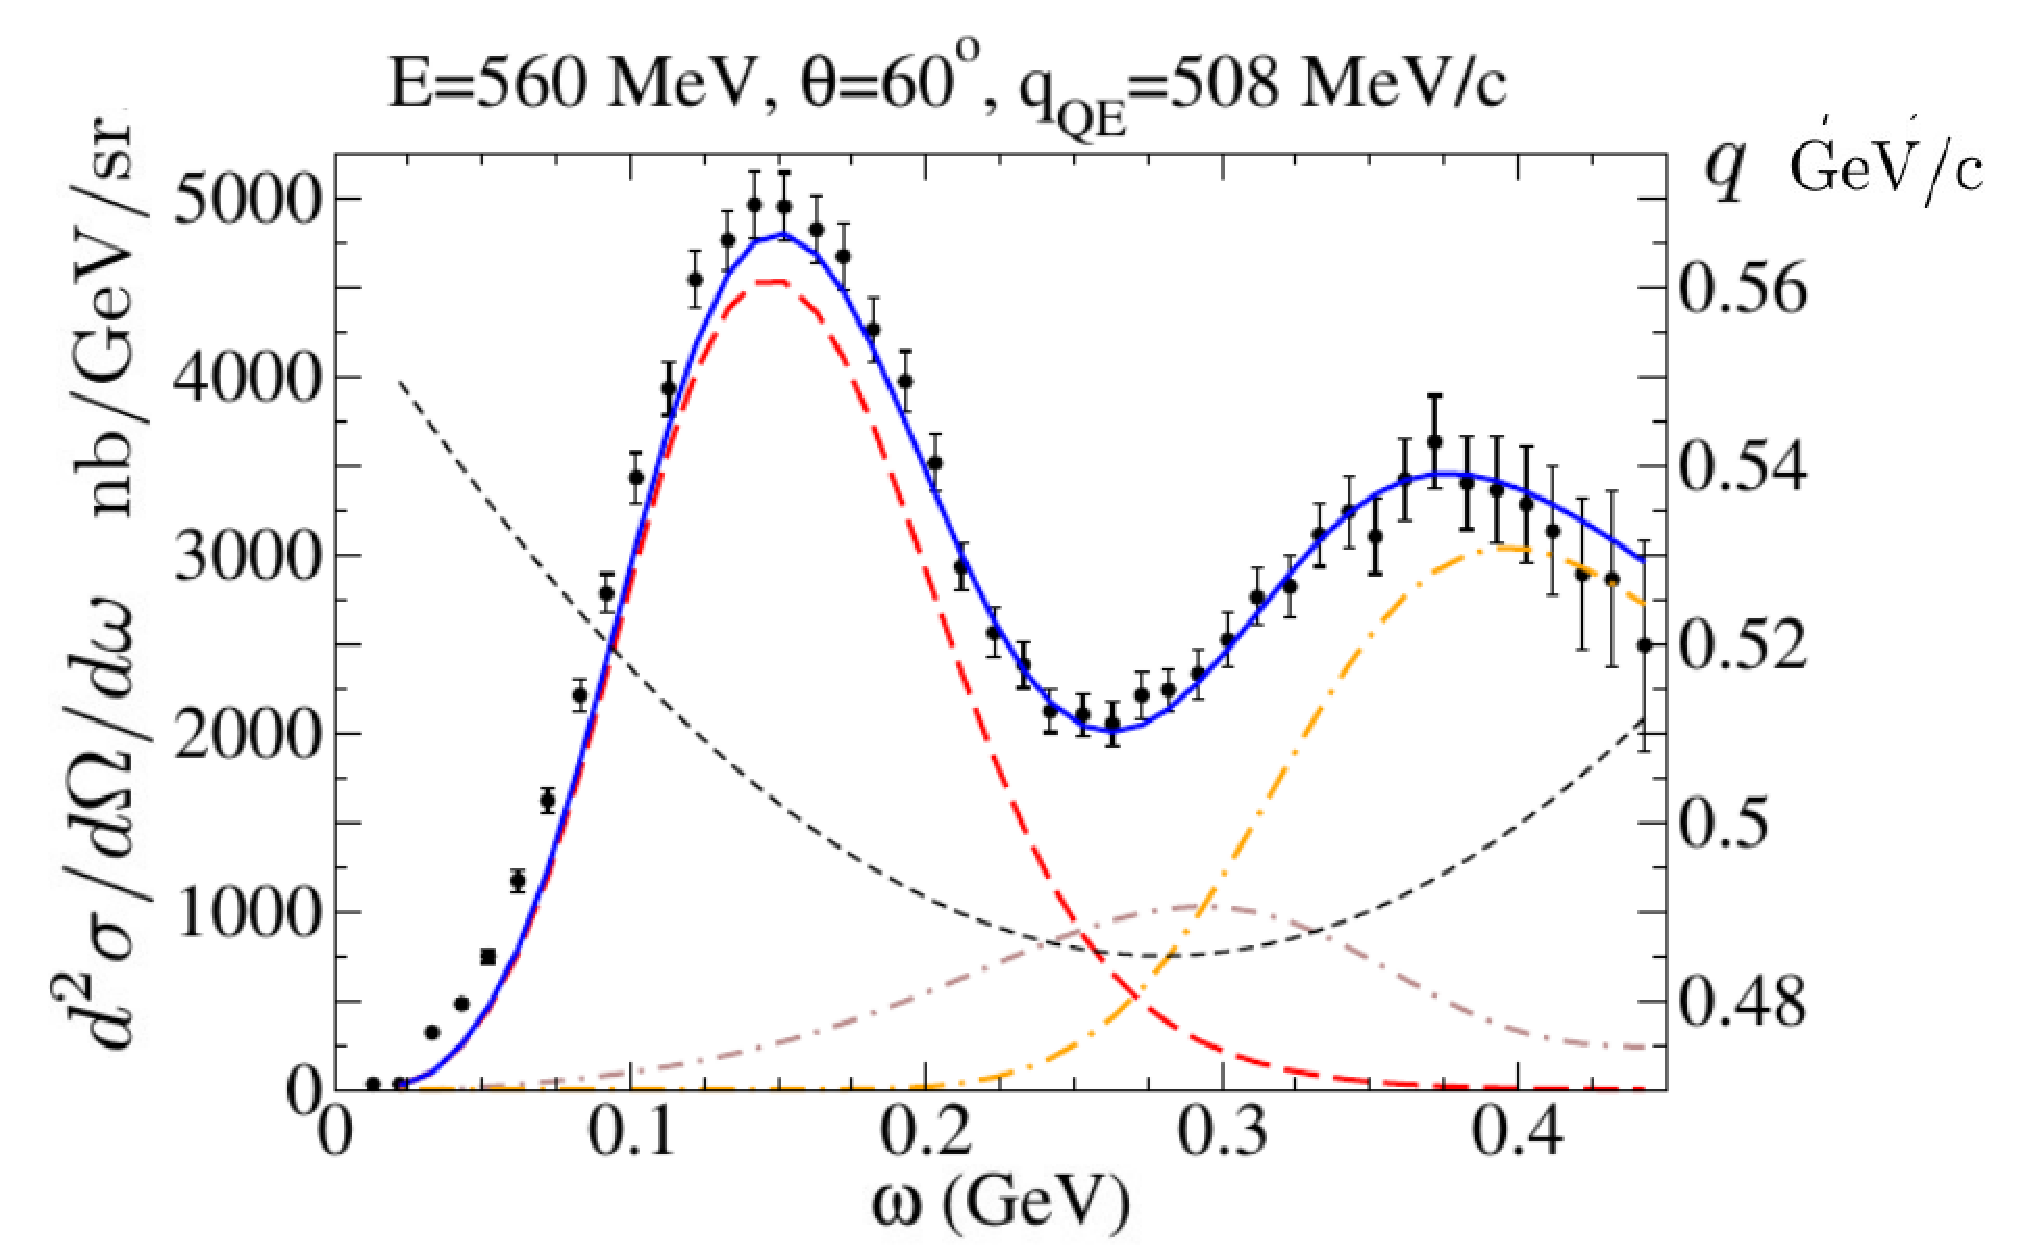
\includegraphics[width=0.6\linewidth]{fig/escattering.pdf}
%\end{center}
%\caption{
%Comparison of inclusive $^{12}$C(e,e') cross sections and predictions of the QE-SuSAv2 model (long-dashed red line), 2p-2h MEC model (dot-dashed brown line) and inelastic-SuSAv2 model (long dot-dashed orange line) (from Ref. \cite{escattering}).
%The sum of the three contributions is represented with a solid blue line.
%The q dependence with $\omega$ is also shown (short-dashed black line.)
%}
%\label{fig:electrono_scattering_data}
%\end{figure}
%
\begin{figure}[tbhp]
\begin{center}
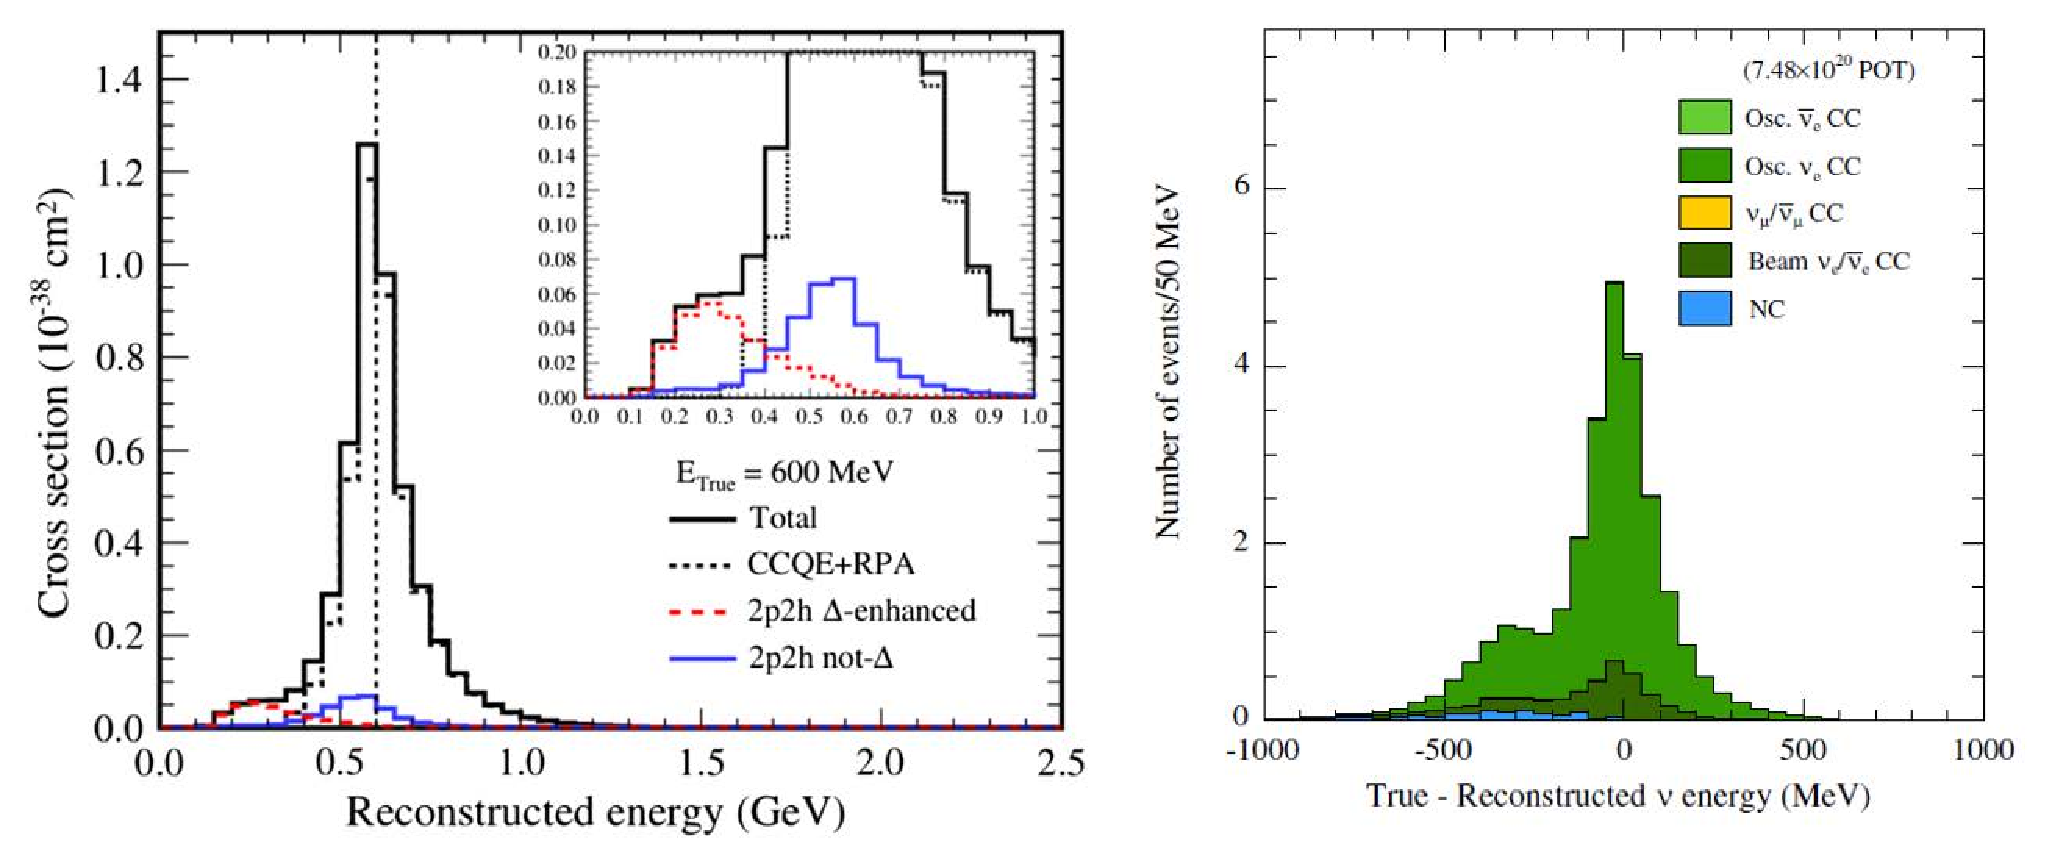
\includegraphics[width=\linewidth]{fig/recE.pdf}
\end{center}
\caption{Left: reconstructed neutrino energy for CCQE and 2p2h interactions of 600~MeV muon neutrinos on $^{12}C$ simulated with a mode.
  Right: difference between true and reconstructed energy of the $\nu_e$ CCQE-like sample.
  The energy is reconstructed from the lepton momentum assuming the kinematics of the CCQE interaction.
  Both plots from \cite{Abe:2017vifw}
}
\label{fig:ene_rec_bias}
\end{figure}
%
\begin{figure}[tbhp]
 \begin{center}
  \begin{subfigure}{0.48\textwidth}
     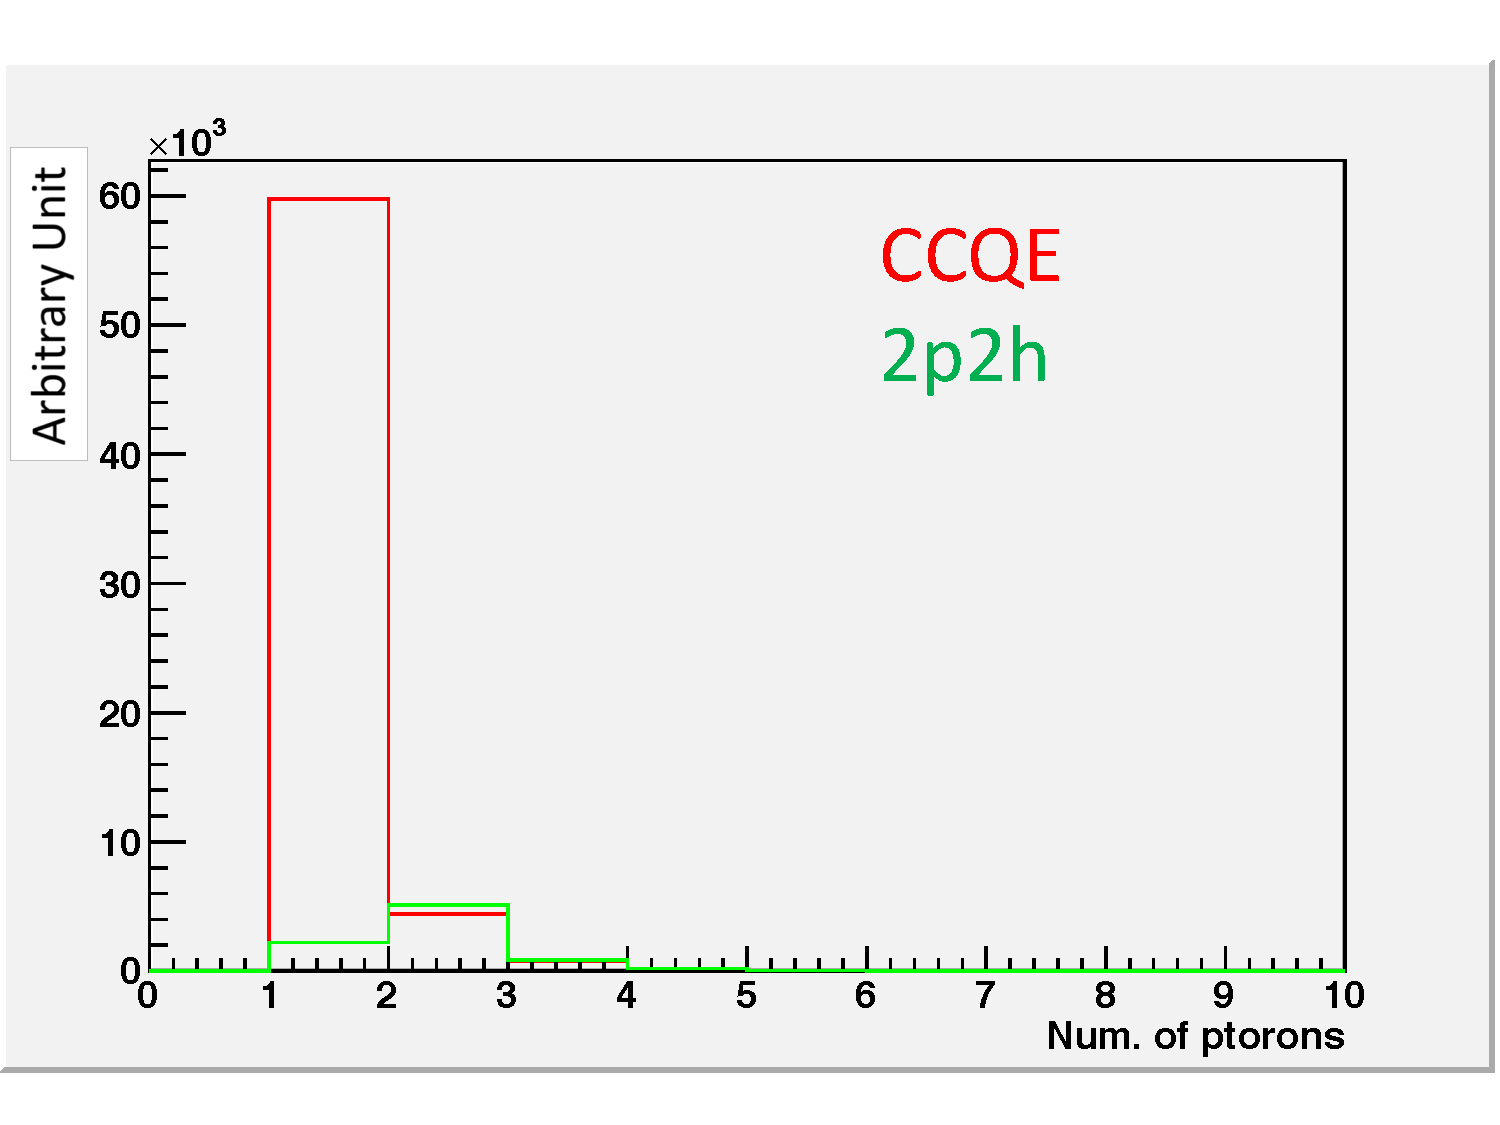
\includegraphics[width=\linewidth]{fig/2p2h_proton_multiplicity.pdf}
    \end{subfigure}
  \begin{subfigure}{0.48\textwidth}
    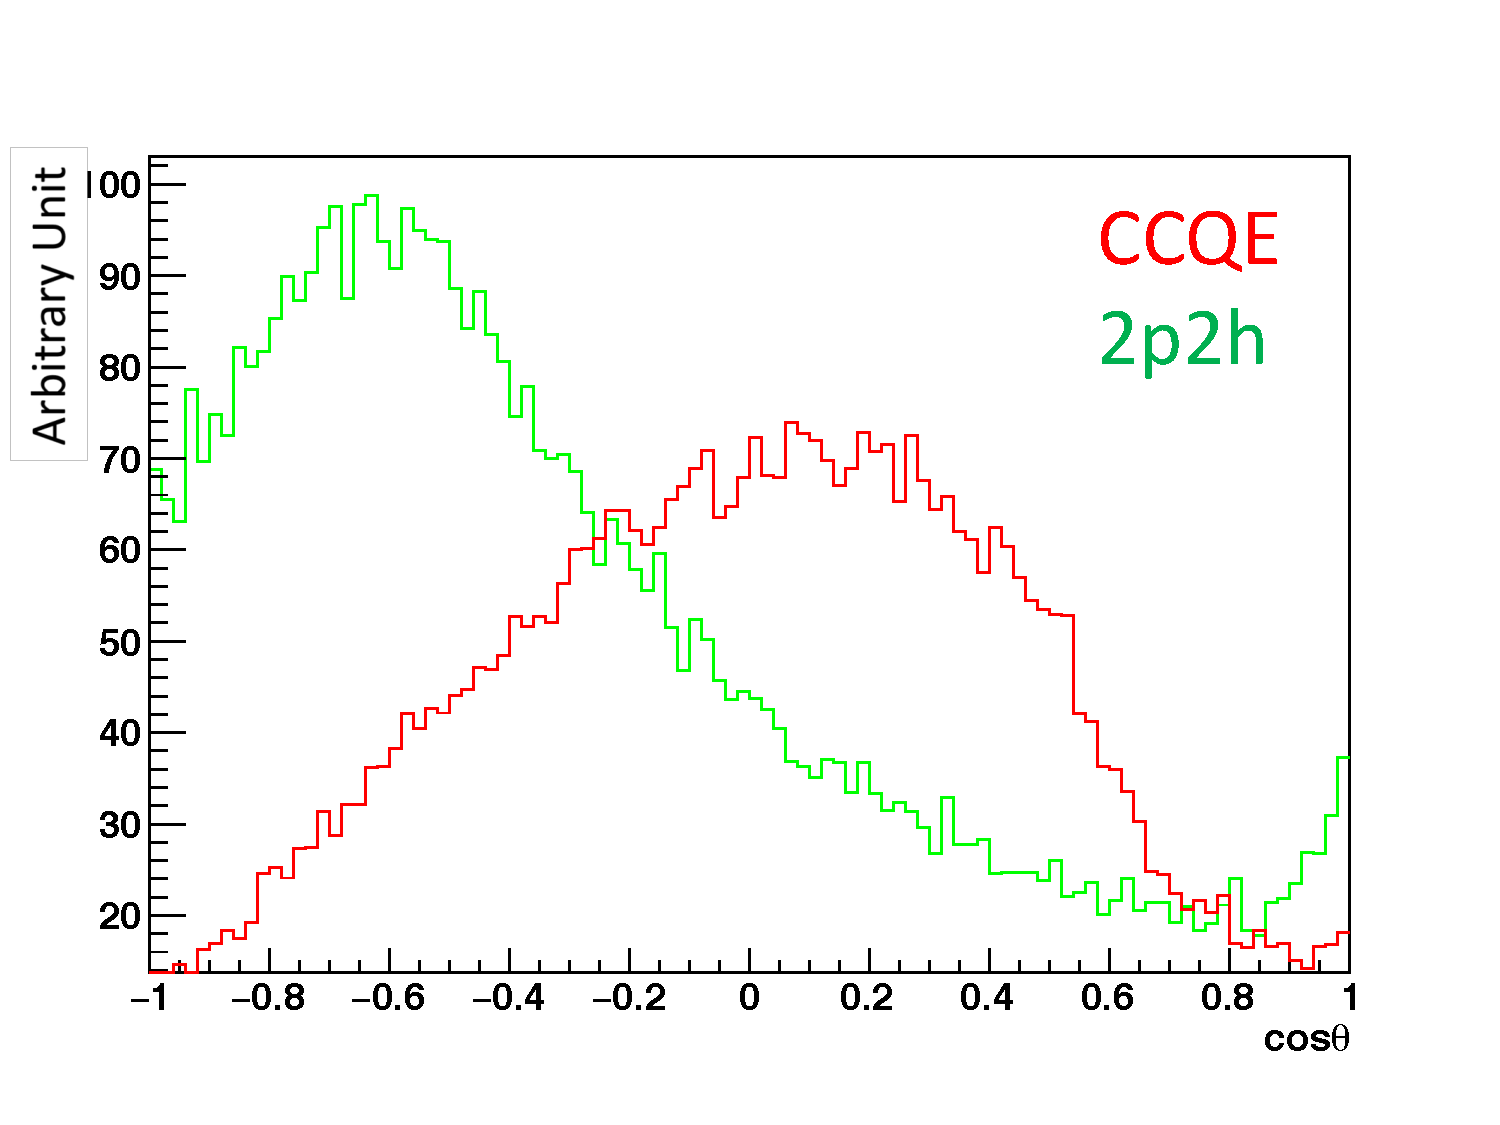
\includegraphics[width=\linewidth]{fig/2p2h_proton_angle.pdf}
    \end{subfigure}    
    \end{center}
  \caption{
Proton multiplicities (left) and opening angles between two proton tracks (right) for CCQE events and 2p2h events.
The final-state interaction is taking into account.
}
\label{fig:2p2h_proton_multiplicity_angle}
\end{figure}


% The corrections from collective nuclear effects calculated by RPA as a function of $Q^{2}$ are shown in Fig. \ref{fig:effect_rpa}.
% The $Q^{2}$ dependence of the correction can be tested by measuring angular distribution of muons in CC1-$\mu$ and CC1-$\mu 1p$ events.
% The uncertainties of the corrections in low (high) $Q^{2}$ regions can be constrained by observing the events with a forward-going (high-angle) muon, so it is essential to measure muon tracks with full acceptance.
There are various models which describe the collective nuclear effects \cite{collective_nuclear_effect}.
The wide acceptance of the WAGASCI experiment will provide information complementary to ND280 and will play important role to select/tune models.
%The $Q^{2}$ dependence of the effects can be tested by measuring angular distribution of muons in CC1-$\mu$ and CC1-$\mu 1p$ events.
%The uncertainties of the effects in low (high) $Q^{2}$ regions can be constrained by observing the events with a forward-going (high-angle) muon, so it is essential to measure muon tracks with full acceptance.
% Based on the measurement, we can evaluate the models and determine model parameters.

T2K is starting to use $\nu_{e}$ CC1$\pi$ samples at the far detector to increase the statistics.
One of the biggest uncertainty of the CC1$\pi$ sample comes from the final state interactions of pions in the nuclei after the initial neutrino interactions because they change the multiplicity, charge and kinematics of the pions.
The multi-pion production events can be migrated into the CC1$\pi$ sample due to the FSIs, and they become backgrounds.
The WAGASCI module has a capability to distinguish the pion track and proton track from d$E$/d$x$, so 
WAGASCI can provide the CC1$\pi$ cross section with low momentum threshold and wide acceptance for pion tracks.
%constrain the uncertainties from the pion FSIs by measuring pion rescattering in the detector and pion multiplicity in $\nu_{\mu}$ CCn$\pi$ sample
%with low detection threshold and full acceptance for pion tracks.
%The water-out WAGASCI can provide good sample for the pion FSI studies because its low density medium enables the detection of low momentum pions in addition to the full acceptance.




